%iffalse
\let\negmedspace\undefined
\let\negthickspace\undefined
\documentclass[journal,12pt,onecolumn]{IEEEtran}
\usepackage{cite}
\usepackage{amsmath,amssymb,amsfonts,amsthm}
\usepackage{algorithmic}
\usepackage{graphicx}
\usepackage{textcomp}
\usepackage{xcolor}
\usepackage{txfonts}
\usepackage{listings}
\usepackage{enumitem}
\usepackage{mathtools}
\usepackage{gensymb}
\usepackage{comment}
\usepackage[breaklinks=true]{hyperref}
\usepackage{tkz-euclide} 
\usepackage{listings}
\usepackage{gvv}                                        
%\def\inputGnumericTable{}                                 
\usepackage[latin1]{inputenc}                                
\usepackage{color}                                            
\usepackage{array}                                            
\usepackage{longtable}                                       
\usepackage{calc}                                             
\usepackage{multirow}                                         
\usepackage{hhline}                                           
\usepackage{ifthen}                                           
\usepackage{lscape}
\usepackage{tabularx}
\usepackage{array}
\usepackage{float}

\usepackage{enumitem}
\usepackage{xcolor}
%\usepackage{multicol}


\newtheorem{theorem}{Theorem}[section]
\newtheorem{problem}{Problem}
\newtheorem{proposition}{Proposition}[section]
\newtheorem{lemma}{Lemma}[section]
\newtheorem{corollary}[theorem]{Corollary}
\newtheorem{example}{Example}[section]
\newtheorem{definition}[problem]{Definition}
\newcommand{\BEQA}{\begin{eqnarray}}
\newcommand{\EEQA}{\end{eqnarray}}
\newcommand{\define}{\stackrel{\triangle}{=}}
\theoremstyle{remark}
\newtheorem{rem}{Remark}

\title{Vector Arithmetic (Section Formula)}
\author{AI24BTECH11021 - Manvik Muthyapu}
\begin{document}
\bibliographystyle{IEEEtran}

\maketitle
\bigskip

\renewcommand{\thefigure}{\theenumi}
\renewcommand{\thetable}{\theenumi}

\textbf{Question}:\\
Show that the points $\textbf{A}\brak{-6,10},\textbf{B}\brak{-4,6}$ and $\textbf{C}\brak{3,-8}$ are collinear such that $AB = \frac{2}{9}AC$.\\
		
\solution 
To prove that the given points are collinear, we check the determinant of the following matrix:

$$
\text{Det} = 
\begin{vmatrix}
-6 & 10 & 1 \\
-4 & 6 & 1 \\
3 & -8 & 1
\end{vmatrix}
$$

If the determinant is zero, then the points $A$, $B$, and $C$ are collinear. Therefore, we have:

$$
\text{Det} = 
\begin{vmatrix}
-6 & 10 & 1 \\
-4 & 6 & 1 \\
3 & -8 & 1
\end{vmatrix}
= 0$$

Thus, $A$, $B$, and $C$ are collinear.\\

We can prove that $AB = \frac{2}{9} AC$ using the section formula.\\

We want to show that $B\brak{-4, 6}$ divides $AC$ in the ratio $2:7$.\\

Using the section formula, if $B$ divides $AC$ in the ratio $m:n$, then:

$$B\brak{\frac{m \cdot 3 + n \cdot (-6)}{m+n}, \frac{m \cdot (-8) + n \cdot 10}{m+n}} = (-4, 6)$$

Equating the coordinates, we get 
$$\frac{m}{n} = \frac{2}{7}$$


Thus, it confirms that $B$ divides $AC$ in the ratio $2:7$.
Since $B$ divides $AC$in the ratio $2:7$, we have:


$$\frac{AB}{AC} = \frac{2}{2+7} = \frac{2}{9}$$

Hence, $AB = \frac{2}{9} AC$, as required.

\begin{figure}[h!]
	\centering
	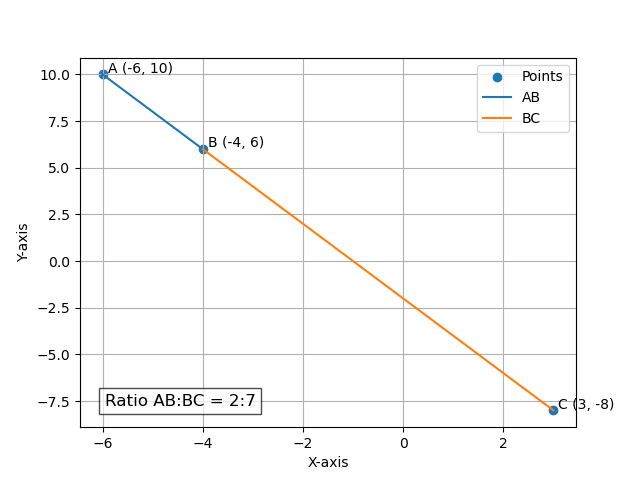
\includegraphics[width=0.7\linewidth]{figs/fig1.png}
\end{figure}
\end{document}


